\section{Magnetic Levitation System}
\label{sec:magnetic_levitation_system}

As stated in the introduction, the system under study is the \acrfull{mls} provided by \texttt{Inteco} (producer vebsite: \url{https://www.inteco.com.pl/products/magnetic-levitation-systems/}).
In Figure \ref{fig:MLS} the system used in this work is shown.

\begin{figure}[H]
    \centering
    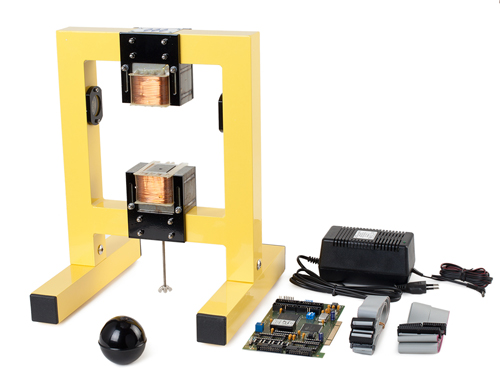
\includegraphics[width=0.7\textwidth]{./img/maglev_picture.jpg}
    \caption{\acrlong{mls}}
    \label{fig:MLS}
\end{figure}

As it can be seen quite clearly, the system is composed of a simple mechanical structure that is used to support two electromagnets and an optical infrared sensor.
Along with the mechanical structure, a ferromagnetic ball and a control unit are present.

At its core principle, the system uses the interaction between the magnetic field generated by the electromagnets and the ferromagnetic ball to keep the ball in a desired position.
The optical sensor is used to measure the position of the ball and provide feedback to the control unit that, in turn, adjusts the voltage applied to (and indeed the current flowing through) the electromagnets to keep the ball in a desired position.
In Figure \ref{fig:MLS_schematic} a schematic representation of the upper half of the system is shown.

\begin{figure}[H]
    \centering
    \begin{minipage}{0.45\textwidth}
        \centering
        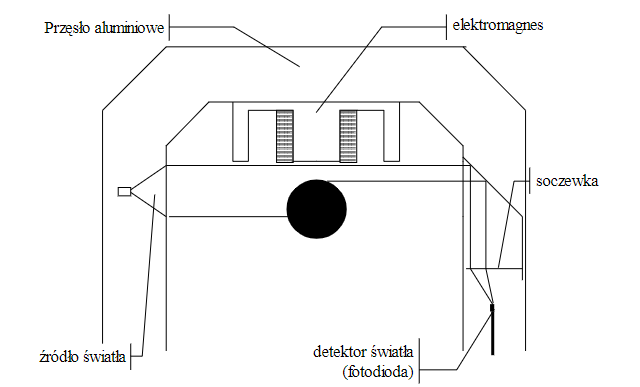
\includegraphics[width=0.9\textwidth]{./img/maglev_scheme.png}
        \caption{Schematic representation of the \acrshort{mls} system.}
        \label{fig:MLS_schematic}
    \end{minipage}
    \hfill
    \begin{minipage}{0.45\textwidth}
        \centering
        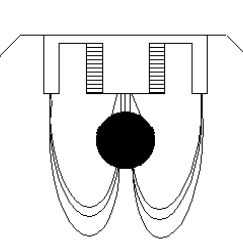
\includegraphics[width=0.9\textwidth]{./img/object_in_magnetic_field.png}
        \caption{Representation of the object in the magnetic field.}
        \label{fig:object_in_magnetic_field}
    \end{minipage}
\end{figure}

\paragraph{Real world application}

Despite the fact that our system is a simplified use case, the magnetic levitation principle is used in many real-world applications.

One of the most common applications is the magnetic levitation trains, also known as `MagLev' trains.
These trains use the magnetic levitation principle to lift the train off the tracks and propel it forward using the magnetic field generated by the tracks.
The main advantage of this technology is the absence of friction between the train and the tracks, which allows the train to reach higher speeds and reduce the noise characteristic of the traditional trains.
Some of the fastest (operating) trains in the world are MagLev trains, with the Shanghai MagLev train being the fastest, reaching a top speed of $623 km/h$ \cite{WikiSCMaglev}.

Another application of the magnetic levitation principle is the magnetic bearings.
These bearings use the magnetic field generated by electromagnets to levitate a rotor and keep it in a desired position.
The main advantage of this technology is the absence of mechanical contact between the rotor and the stator, which allows the rotor to reach higher speeds and reduce the wear of the components.

\subsection{Model derivation}
\label{subsec:model_derivation}

The \acrshort{mls} is a complex system that can be divided into two main subsystems:

\begin{itemize}
    \item \textbf{Electromagnetic subsystem}: it takes into account the electrical components of the system from the power supply to the generation of the magnetic field by the coils;
    \item \textbf{Mechanical subsystem}: it takes into account the dynamics of the ball and all the forces acting on it, including the electromagnetic forces generated by the magnetic field.
\end{itemize}

Due to the presence of the ball that moves inside a magnetic field, a complex connection between the two subsystems that goes beyond the simple force balance exists.
For this reason, it's almost impossible to derive a complete model without considering both subsystems at the same time.

In Figure \ref{fig:system_model}, a schematic representation of all the components and forces acting on the system is shown.
Instead, in Table \ref{tab:components} a brief description of the components of the system and their units is reported.

\begin{figure}[H]

    \begin{minipage}{0.40\textwidth}

        \centering

        \begin{tikzpicture}[european voltages]

            \def\radius{0.3}

            % Upper circuit
            \node at (-1.0, 3.5) {$T_1$};
            \draw (-3, 3.5) node [right] {$+$}
            to [short] ++(0, -1)
            to [R, l^=$R_1$, resistors/zigs=6] ++(2, 0)
            to [variable cute inductor, i>^=$I_1$, l=$L_1$] ++(2, 0)
            to [short] ++(0, +1) node [right] {$-$};

            % Reference system
            \draw[|->] (-1.0, +2.5) -- ++(0, -3) node[left] {$z$, $\dot{z}$, $\ddot{z}$};

            % Ball
            \filldraw[fill=gray, draw=black] (0, 0) circle (\radius);

            % Upward forces
            \draw[thick, ->] (-0.1, +\radius) -- ++(0, +1.5) node[right] {$F_{\text{em1}}$};
            \draw[thick, ->] (+0.0, +\radius) -- ++(0, +1.0) node[right] {$F_{\text{in}}$};
            \draw[thick, ->] (+0.1, +\radius) -- ++(0, +0.5) node[right] {$F_{\text{d}}$};

            % Downward forces
            \draw[thick, ->] (+0.1, -\radius) -- ++(0, -0.5) node[right] {$F_{\text{g}}$};
            \draw[thick, ->] (-0.1, -\radius) -- ++(0, -1.0) node[right] {$F_{\text{em2}}$};

            % Lower circuit
            \node at (-1.0, -3.0) {$T_2$};
            \draw (-3, -3) node [right] {$+$}
            to [short] ++(0, +1)
            to [R, l_=$R_2$, resistors/zigs=6] ++(2, 0)
            to [variable cute inductor, i>_=$I_2$, l_=$L_2$] ++(2, 0)
            to [short] ++(0, -1) node [right] {$-$};

        \end{tikzpicture}

    \end{minipage}
    %
    \hfill
    %
    \begin{minipage}{0.55\textwidth}

        \centering

        \begin{tabular}{|c|l|c|}
            \hline
            \textbf{Name}      & \textbf{Description}             & \textbf{Units} \\
            \hline
            $F_{\text{g}}$     & Gravitational force              & N              \\
            $F_{\text{in}}$    & Inertial force                   & N              \\
            $F_{\text{d}}$     & Drag force                       & N              \\
            $F_{\text{em1,2}}$ & Electromagnetic force            & N              \\
            $R_{1,2}$          & Resistance of the coil           & $\Omega$       \\
            $L_{1,2}$          & Inductance of the coil           & H              \\
            $I_{1,2}$          & Current flowing through the coil & A              \\
            $V_{1,2}$          & Voltage applied to the coil      & V              \\
            $T_{1,2}$          & Temperature of the coil          & $^\circ C$     \\
            \hline
        \end{tabular}

    \end{minipage}

    \caption{Schematic representation of the \acrshort{mls} system and description of the components.}
    \label{fig:system_model}
    \label{tab:components}

\end{figure}


In the following sections, we will derive the equations that governs the \acrshort{mls} system, adopting an energetic approach that starts from the energy conservation principle.

\subsubsection{Mathematical model}
\label{subsubsec:mathematical_model}

We can now proceed with the derivation of the equations that govern the system.

At first, we can recall that the energy conservation principle states that the sum of the kinetic, potential, and dissipated energy of the system is equivalent to the work done by the external forces acting on the system.

\paragraph{Lagrange's equation}

Thanks to the Lagrange's equation we write the following, that encaptulates the energy conservation principle:

\begin{equation}
    \frac{d}{dt} \left( \frac{\partial \mathcal{T}}{\partial \dot{\mathbf{u}}} \right) - \frac{\partial \mathcal{T}}{\partial \mathbf{u}} + \frac{\partial \mathcal{D}}{\partial \dot{\mathbf{u}}} + \frac{\partial \mathcal{U}}{\partial \mathbf{u}} = \mathcal{Q}
    \label{eq:lagrange_equation}
\end{equation}

Where $\mathbf{u}$ is the generalized coordinates of the system, $\mathbf{T}$ is the kinetic energy of the system, $\mathbf{D}$ is the dissipated energy of the system, $\mathbf{U}$ is the potential energy of the system, and $\mathbf{Q}$ is the generalized input to the system.

At first, we can give a definition of all the energetic terms included in Equation \ref{eq:lagrange_equation} for the \acrshort{mls} system.
Notice that with respect to traditional purely mechanical systems, we also have to consider the stored energy in the coils as inductors, the dissipation due to the resistance of the coils, and the potential energy given by the external power supply.

By doing so, we can write the kinetic energy of the system as:

\begin{equation}
    \mathcal{T} = \frac{1}{2} m \dot{z}^2 + \frac{1}{2} L_1(z, T_1) \dot{q_1}^2 + \frac{1}{2} L_2(z, T_2) \dot{q_2}^2
    \label{eq:kinetic_energy}
\end{equation}

Where $m$ is the mass of the ball, $L_1$ and $L_2$ are the inductances of the coils, and $q_1$ and $q_2$ are the charges stored in the coils.
It follows that $\dot{q_1}$ and $\dot{q_2}$ are the currents flowing through the coils.

The dissipated energy of the system can be written as:

\begin{equation}
    \mathcal{D} = \int_{\dot{z}(\cdot)} \frac{1}{2} C_d A \rho \dot{z}^2 d\dot{z} + \int_{\dot{q_1}(\cdot)} R_1(T_1) \dot{q_1} d\dot{q_1} + \int_{\dot{q_2}(\cdot)} R_2(T_2) \dot{q_2} d\dot{q_2}
    \label{eq:dissipated_energy}
\end{equation}

Where $C_d$ is the drag coefficient, $A$ is the cross-sectional area of the ball, and $\rho$ is the density of the air.

Instead, the potential energy of the system can be written as:

\begin{equation}
    \mathcal{U} = -m g z - q_1 V_1 - q_2 V_2
    \label{eq:potential_energy}
\end{equation}

Where $V_1$ and $V_2$ are the voltages applied to the coils.

Finally, the generalized input to the system can be evaluated as:

\begin{equation}
    \mathcal{Q} = 0
    \label{eq:generalized_input}
\end{equation}

For convenience, we have chosen to consider both the external power supplied to the coils and the gravitational force as potential energy terms and not as generalized inputs.
Notice also the minus sign in the potential energy term, which is due to the fact that the gravitational force increases the potential energy with respect to the chosen reference frame (positive downwards).

\paragraph{Temperature dependence components}

Before proceeding, it's necessary to explicitly the dependence of the inductance and resistance terms on the temperature of the coils.
However, we can assume that in first approximation the sensitivity of both the electrical components to the temperature is negligible.
This is strong and possibly incorrect assumption, but it allows us to simplify the model and focus on the main dynamics of the system.

For the assumption stated above, we can write the resistance terms as:

\begin{equation}
    \begin{aligned}
        R_1 & = R_1(T_1) = R_{10} \\
        R_2 & = R_2(T_2) = R_{20}
    \end{aligned}
    \label{eq:resistance}
\end{equation}

Where $R_{*0}$ are the resistances of the coils at ambient temperature with negligible current flowing through them.

Instead, we can write the inductance terms as:

\begin{equation}
    \begin{aligned}
        L_1 & = L_1(z, T_1) = L_{10} + L_{1z} e^{-a_1 z}            \\
        L_2 & = L_2(z, T_2) = L_{20} + L_{2z} e^{-a_2 (h - 2r - z)}
    \end{aligned}
    \label{eq:inductance}
\end{equation}

Where $L_{*0}$ are the inductances when no objects are present in the magnetic field volume, while $L_{*z}$ and $a_*$ are coefficients that take into account the variation of the inductance due to the presence of the ball in the magnetic field.

\paragraph{Equations of motion}

To derive the equations of motion of the system, we can substitute the kinetic, potential, and dissipated energy terms into the Lagrange's equation \ref{eq:lagrange_equation}.
Notice that by analyzing the system, we can see that the generalized coordinates are $z$, $q_1$, and $q_2$, and so the vector of generalized coordinates is $\mathbf{u} = [z, q_1, q_2]^T$.

Once $\mathbf{u}$ has been identify, the procedure to derive the equations of motion is straightforward.
Following Equation \ref{eq:lagrange_equation}, we can write the following system of equations:

\begin{equation}
    \begin{cases}
        \frac{d}{dt} \left( \frac{\partial \mathcal{T}}{\partial \dot{z}} \right) - \frac{\partial \mathcal{T}}{\partial z} + \frac{\partial \mathcal{D}}{\partial \dot{z}} + \frac{\partial \mathcal{U}}{\partial z} = \mathcal{Q}         \\
        \frac{d}{dt} \left( \frac{\partial \mathcal{T}}{\partial \dot{q_1}} \right) - \frac{\partial \mathcal{T}}{\partial q_1} + \frac{\partial \mathcal{D}}{\partial \dot{q_1}} + \frac{\partial \mathcal{U}}{\partial q_1} = \mathcal{Q} \\
        \frac{d}{dt} \left( \frac{\partial \mathcal{T}}{\partial \dot{q_2}} \right) - \frac{\partial \mathcal{T}}{\partial q_2} + \frac{\partial \mathcal{D}}{\partial \dot{q_2}} + \frac{\partial \mathcal{U}}{\partial q_2} = \mathcal{Q}
    \end{cases}
\end{equation}

By substituting the energetic terms obtained in Equations \ref{eq:kinetic_energy}, \ref{eq:dissipated_energy}, \ref{eq:potential_energy}, \ref{eq:generalized_input} into the set of equations above, we obtain the following equations of motion:

\begin{equation}
    \begin{cases}
        m \ddot{z} - \frac{1}{2} \frac{\partial L_1}{\partial z} \dot{q_1}^2 - \frac{1}{2} \frac{\partial L_2}{\partial z} \dot{q_2}^2 + \frac{1}{2} C_d A \rho \dot{z}^2 - m g = 0 \\
        L_1 \ddot{q_1} + \frac{\partial L_1}{\partial z} \dot{z} \dot{q_1} + R_1 \dot{q_1} - V_1 = 0                                                                                \\
        L_2 \ddot{q_2} + \frac{\partial L_2}{\partial z} \dot{z} \dot{q_2} + R_2 \dot{q_2} - V_2 = 0
    \end{cases}
\end{equation}

For convenience, we can transform the second order differential equations into first order differential equations by introducing a fourth equation in the set above and considering the currents as state variables.

\begin{equation}
    \begin{cases}
        \dot{z} = v                                                                                                                                                                    \\
        \dot{v} = m^{-1} \left(\frac{1}{2} \frac{\partial L_1}{\partial z} I_1^2 + \frac{1}{2} \frac{\partial L_2}{\partial z} I_2^2 - \frac{1}{2} C_d A \rho \dot{z}^2 + m g  \right) \\
        \dot{I_1} = L_1^{-1} \left(- \frac{\partial L_1}{\partial z} \dot{z} I_1 - R_1 I_1 + V_1 \right)                                                                               \\
        \dot{I_2} = L_2^{-1} \left(- \frac{\partial L_2}{\partial z} \dot{z} I_2 - R_2 I_2 + V_2 \right)
    \end{cases}
    \label{eq:equations_of_motion}
\end{equation}

The set of equations above represents the complete mathematical model of the \acrshort{mls} system.
One can notice that the equations are both nonlinear and coupled, making the system hard to analyze and control.

\paragraph{Neglecting velocity terms}

In the optics of simplifying the model and making it easier to analyze and control, we can neglect all the terms in Equation \ref{eq:equations_of_motion} that are linearly dependent on the velocity of the ball.
This assumption is reasonable due to the fact that the velocity of the ball (as also reported in later section of the report) will never be grater that a few centimeters per second.
This means that, considering $\dot{z} \approx 10 [mm/s]$, we can write the following inequality:

\begin{equation}
    \begin{aligned}
        \left| -\frac{1}{2} C_d A \rho \dot{z}^2 \right|            & << m g \\
        \left| -\frac{\partial L_1}{\partial z} \dot{z} I_1 \right| & << V_1 \\
        \left| -\frac{\partial L_2}{\partial z} \dot{z} I_2 \right| & << V_2
    \end{aligned}
\end{equation}

By doing so, we can simplify the equations of motion as:

\begin{equation}
    \begin{cases}
        \dot{z} = v                                                                                                                                 \\
        \dot{v} = m^{-1} \left(\frac{1}{2} \frac{\partial L_1}{\partial z} I_1^2 + \frac{1}{2} \frac{\partial L_2}{\partial z} I_2^2 + m g  \right) \\
        \dot{I_1} = L_1^{-1} \left(- R_1 I_1 + V_1 \right)                                                                                          \\
        \dot{I_2} = L_2^{-1} \left(- R_2 I_2 + V_2 \right)
    \end{cases}
    \label{eq:equations_of_motion_no_velocity}
\end{equation}


\subsubsection{Literature model}
\label{subsubsec:literature_model}

In the literature, the model of the \acrshort{mls} system is often further simplified by considering empirical values associated with the inductances and resistances of the coils.
In particular, starting from the just derived model in Equation \ref{eq:equations_of_motion_no_velocity}, one can rewrite currents dynamics as:

\begin{equation}
    \begin{aligned}
        \dot{I_1} & = \frac{R_1}{L_1} \left(- I_1 + \frac{V_1}{R_1} \right) \\
        \dot{I_2} & = \frac{R_2}{L_2} \left(- I_2 + \frac{V_2}{R_2} \right)
    \end{aligned}
\end{equation}

Moreover, from experimental data performed on the system, one can derive the following empirical relations, valid at least in the region of interest:

\begin{equation}
    \begin{aligned}
        \frac{L_1}{R_1} & \approx f_1(z) = \frac{f_{IP1}}{f_{IP2}} e^{\left(-\frac{z}{f_{IP2}}\right)}          \\
        \frac{L_2}{R_2} & \approx f_2(z) = \frac{f_{IP1}}{f_{IP2}} e^{\left(-\frac{h - 2r - z}{f_{IP2}}\right)}
    \end{aligned}
    \label{eq:empirical_relations}
\end{equation}


\subsubsection{Black zone control}
\label{subsubsec:black_zone_control}

A final important remark has to be made about the so-called \textit{black zone} of the system, that are the regions where the current flowing through the coils is no more reachable.

In particular, by simply connect the power supply to the coils, a minimum voltage will be applied and a certain amount of current will flow through the coils.
In the following, we will refer to this current and voltage as $I_{*min}$ and $V_{*min}$ respectively.

Because of this, the above derived model (Equation \ref{eq:equations_of_motion_no_velocity} and Equation \ref{eq:empirical_relations}) must be slightly modified to take into account the black zone of the system.

In particular, Equation \ref{eq:equations_of_motion_no_velocity} can be rewritten as:

\begin{equation}
    \begin{cases}
        \dot{z} = v                                                                                                                                 \\
        \dot{v} = m^{-1} \left(\frac{1}{2} \frac{\partial L_1}{\partial z} I_1^2 + \frac{1}{2} \frac{\partial L_2}{\partial z} I_2^2 + m g  \right) \\
        \dot{I_1} = L_1^{-1} \left(- R_1 I_1 + V_1 + V_{1min} \right)                                                                               \\
        \dot{I_2} = L_2^{-1} \left(- R_2 I_2 + V_2 + V_{2min} \right)
    \end{cases}
    \label{eq:equations_of_motion_no_velocity_final}
\end{equation}

While Equation \ref{eq:empirical_relations} can be rewritten as:

\begin{equation}
    \begin{aligned}
        \dot{I_1} & = \frac{R_1}{L_1} \left(- I_1 + \frac{V_1}{R_1} + I_{1min} \right) \\
        \dot{I_2} & = \frac{R_2}{L_2} \left(- I_2 + \frac{V_2}{R_2} + I_{2min} \right)
    \end{aligned}
\end{equation}
\subsection{Model Linearization}
\label{subsec:model_linearization}

\hl{We need to write how the operating point vector has been computed}

The model derived in the previous subsection is highly non-linear.
In order to begin able to apply linear control techniques, it is necessary to linearize the model around a given operating point.

From now on, we will suppose the operating point as:

\begin{equation}
    \mathbf{x}_{op} =
    \begin{bmatrix}
        z_{op}     \\
        v_{op} = 0 \\
        I_{1op}    \\
        I_{2op}    \\
        U_{1op}    \\
        U_{2op}
    \end{bmatrix}
\end{equation}

By doing so, the linearized model can be obtained by performing a Taylor expansion around the operating point up to the first order terms of Equations \ref{eq:reduced_equations_of_motion_final} or Equations \ref{eq:simplified_equations_of_motion_final}.

Before performing the linearization, we briefly recall the general form of a Taylor expansion of a function $f(\mathbf{x})$ around a point $\mathbf{x}_{op}$:

\begin{equation}
    f(\mathbf{x}) \approx f(\mathbf{x}_{op}) + \nabla f(\mathbf{x}_{op}) \cdot (\mathbf{x} - \mathbf{x}_{op})
\end{equation}

Where $\nabla f(\mathbf{x}_{op})$ is the gradient of $f(\mathbf{x})$ evaluated at $\mathbf{x}_{op}$.

By applying the Taylor expansion to the non-linear model, the linearized model can be obtained as:

\begin{equation}
    \mathbf{f}(\mathbf{x}) - \mathbf{f}(\mathbf{x}_{op})\approx \frac{\partial \mathbf{f}}{\partial \mathbf{x}} \Bigg|_{\mathbf{x}_{op}} \cdot (\mathbf{x} - \mathbf{x}_{op})
\end{equation}

Considering now the set of Equations \ref{eq:reduced_equations_of_motion_final}, the linearized model can be obtained as:

\begin{equation}
    \begin{cases}
        \dot{z} - \dot{z_{op}}    & \approx 1 (v - v_{op})                  \\
        \dot{v} - \dot{v_{op}}    & \approx m^{-1} \left(
        \frac{1}{2} \frac{\partial^2 L_1}{\partial z^2} \Bigg|_{\mathbf{x}_{op}} (z - z_{op}) I_{1op}^2 +
        \frac{1}{2} \frac{\partial^2 L_2}{\partial z^2} \Bigg|_{\mathbf{x}_{op}} (z - z_{op}) I_{2op}^2 +
        \frac{\partial L_1}{\partial z} \Bigg|_{\mathbf{x}_{op}} I_{1op} (I_1 - I_{1op}) +
        \frac{\partial L_2}{\partial z} \Bigg|_{\mathbf{x}_{op}} I_{2op} (I_2 - I_{2op})
        \right)                                                             \\
        \dot{I_1} - \dot{I_{1op}} & \approx
        \left(- L_1^{-2} \frac{\partial L_1}{\partial z} \left(- R_1 I_1 + k_1 U_1 + c_1 \right) \right) \Bigg|_{\mathbf{x}_{op}} (z - z_{op}) +
        \left(- L_1^{-1} R_1 \right) \Bigg|_{\mathbf{x}_{op}} (I_1 - I_{1op}) +
        \left(L_1^{-1} k_1 \right) \Bigg|_{\mathbf{x}_{op}} (U_1 - U_{1op}) \\
        \dot{I_2} - \dot{I_{2op}} & \approx
        \left(- L_2^{-2} \frac{\partial L_2}{\partial z} \left(- R_2 I_2 + k_2 U_2 + c_2 \right) \right) \Bigg|_{\mathbf{x}_{op}} (z - z_{op}) +
        \left(- L_2^{-1} R_2 \right) \Bigg|_{\mathbf{x}_{op}} (I_2 - I_{2op}) +
        \left(L_2^{-1} k_2 \right) \Bigg|_{\mathbf{x}_{op}} (U_2 - U_{2op})
    \end{cases}
    \label{eq:linearized_model}
\end{equation}

Notice that in the derivation of the linearized model, another model reduction has been performed based on the same assumptions made in the previous subsection with the set of Equations \ref{eq:model_reduction_conditions}.


\subsection{State Space Representation}
\label{subsec:state_space_representation}

\hl{We need to write how the operating point vector has been computed}

In the optics of control theory, it is useful to represent the system in the state space form.
The state space representation is a mathematical model of a physical system as a set of input, output and state variables related by first-order differential equations.
The state space representation is particularly useful for linear systems, as it allows to easily apply linear control techniques.

A generic nonlinear system can be represented in the state space form as:

\begin{equation}
    \begin{aligned}
        \dot{\mathbf{x}} & = f(\mathbf{x}, \mathbf{u}) \\
        \mathbf{y}       & = g(\mathbf{x}, \mathbf{u})
    \end{aligned}
\end{equation}

Where $\mathbf{x}$ is the state vector and $\mathbf{u}$ is the input vector.

Similarly to what has been done in the previous subsection, we can perform a linearization of the system around an operating point to obtain the linearized state space representation in the form of:

\begin{equation}
    \begin{aligned}
        \dot{\delta\mathbf{x}} & \approx A \delta\mathbf{x} + B \delta\mathbf{u} \\
        \delta\mathbf{y}       & \approx C \delta\mathbf{x} + D \delta\mathbf{u}
    \end{aligned}
\end{equation}

Where $\delta\mathbf{x}$ and $\delta\mathbf{u}$ are the deviations of the state and input vectors from the operating point, respectively.
While the matrices $A$, $B$, $C$ and $D$ are the Jacobian matrices with respect to the state and input vectors evaluated at the operating point.

\paragraph{MagLev System State Space Representation}

Given the linearized model derived in the previous subsection, we can define the state vector $\mathbf{x}$ and the input vector $\mathbf{u}$ as:

\begin{equation}
    \mathbf{x} = \begin{bmatrix}
        z   \\
        v   \\
        I_1 \\
        I_2
    \end{bmatrix}
    \quad
    \mathbf{u} = \begin{bmatrix}
        U_1 \\
        U_2
    \end{bmatrix}
\end{equation}

Once the state and input vectors have been defined, the linearized state space representation can be obtained by leveraging the linearized model derived in the previous subsection.
The matrices $A$, $B$, $C$ and $D$ are then defined as:

\begin{equation}
    \begin{aligned}
        A & = \frac{\partial f}{\partial \mathbf{x}} \Bigg|_{(\mathbf{x}_{op}, \mathbf{u}_{op})}
        = \begin{bmatrix}
              0      & 1 & 0      & 0      \\
              a_{21} & 0 & a_{23} & a_{24} \\
              a_{31} & 0 & a_{33} & 0      \\
              a_{41} & 0 & 0      & a_{44}
          \end{bmatrix}                                                           \\
        B & = \frac{\partial f}{\partial \mathbf{u}} \Bigg|_{(\mathbf{x}_{op}, \mathbf{u}_{op})}
        = \begin{bmatrix}
              0      & 0      \\
              0      & 0      \\
              b_{31} & 0      \\
              0      & b_{42}
          \end{bmatrix}                                                                        \\
        C & = \frac{\partial g}{\partial \mathbf{x}} \Bigg|_{(\mathbf{x}_{op}, \mathbf{u}_{op})}
        = \begin{bmatrix}
              1 & 0 & 0 & 0
          \end{bmatrix}                                                                         \\
        D & = \frac{\partial g}{\partial \mathbf{u}} \Bigg|_{(\mathbf{x}_{op}, \mathbf{u}_{op})}
        = \begin{bmatrix}
              0 & 0
          \end{bmatrix}
    \end{aligned}
\end{equation}

By leveraging the linearization of the model derived in the previous subsection and reported in Equation \ref{eq:linearized_model}, the elements of the matrices $A$, $B$, $C$ and $D$ can be computed as:

\begin{equation}
    \begin{aligned}
        a_{21} & = \frac{1}{m} \left( \frac{1}{2} \frac{\partial^2 L_1}{\partial z^2} I_1^2 + \frac{1}{2} \frac{\partial^2 L_2}{\partial z^2} I_{2}^2 \right) \bigg|_{(\mathbf{x}_{op}, \mathbf{u}_{op})} \\
        a_{23} & = \frac{1}{m} \left( \frac{\partial L_1}{\partial z} I_1\right) \bigg|_{(\mathbf{x}_{op}, \mathbf{u}_{op})}                                                                              \\
        a_{24} & = \frac{1}{m} \left( \frac{\partial L_2}{\partial z} I_2\right) \bigg|_{(\mathbf{x}_{op}, \mathbf{u}_{op})}                                                                              \\
        a_{31} & = \left(- L_1^{-2} \frac{\partial L_1}{\partial z} \left(- R_1 I_1 + k_1 U_1 + c_1 \right) \right) \bigg|_{(\mathbf{x}_{op}, \mathbf{u}_{op})}                                           \\
        a_{33} & = \left(L_1^{-1} (-R_1) \right) \big|_{(\mathbf{x}_{op}, \mathbf{u}_{op})}                                                                                                               \\
        a_{41} & = \left(- L_2^{-2} \frac{\partial L_2}{\partial z} \left(- R_2 I_2 + k_2 U_2 + c_2 \right) \right) \bigg|_{(\mathbf{x}_{op}, \mathbf{u}_{op})}                                           \\
        a_{44} & = \left(L_2^{-1} (-R_2) \right) \big|_{(\mathbf{x}_{op}, \mathbf{u}_{op})}                                                                                                               \\
        b_{31} & = \left(L_1^{-1} k_1 \right) \big|_{(\mathbf{x}_{op}, \mathbf{u}_{op})}                                                                                                                  \\
        b_{42} & = \left(L_2^{-1} k_2 \right) \big|_{(\mathbf{x}_{op}, \mathbf{u}_{op})}
    \end{aligned}
\end{equation}



\subsection{Parameters identification}
\label{subsec:parameters_identification}

In order to control the system, we need to identify its parameters.

To do so, different tests type will be performed, such as:

\begin{enumerate}
    \item Direct measurement: measure all the quantity of the system that can be directly measured or retrieved from well established literature;
    \item Control to voltage: observe the relation between the control signal and the effective voltage applied to the coils;
    \item Inductances characterization: identify all the parameters needed to characterize inductances, based on the model proposed in Equation \ref{eq:model_for_inductance};
    \item Force validation: measure the force applied to the ball by the inductance in order to validate both the model and the parameters identified in the previous tests.
\end{enumerate}

Except for the first test, all the others will be performed leveraging the data acquisition system included in the \texttt{Inteco} control unit.

\subsubsection{Direct measurement}
\label{subsubsec:direct_measurement}

In this section, we will measure all the quantities that can be directly measured or retrieved from well established literature.

Most of the following parameters can be directly measured using a scale and a caliper, respectively.
By doing so, we will have the following values:

\begin{table}[H]

    \centering
    \begin{tabular}{|c|c|c|}
        \hline
        \textbf{Parameter} & \textbf{Value} & \textbf{Units} \\
        \hline
        $g$                & $9.81$         & $m/s^2$        \\
        $m$                & $0.06157$      & $kg$           \\
        $r$                & $0.06125/2$    & $m$            \\
        $H$                & $0.098$        & $m$            \\
        \hline
    \end{tabular}

    \caption{Directly measured parameters and constants}
    \label{tab:directly_measured_parameters}

\end{table}

Also from literature, and in particular from the datasheet of the \texttt{Inteco} control unit, we can retrieve the following values about the literature model proposed in Equation \ref{eq:simplified_equations_of_motion_final}:

\begin{table}[H]

    \centering
    \begin{tabular}{|c|c|c|}
        \hline
        \textbf{Parameter} & \textbf{Value}         & \textbf{Units} \\
        \hline
        $F_{emP1}$         & $1.7521 \cdot 10^{-2}$ & $H$            \\
        $F_{emP2}$         & $5.8231 \cdot 10^{-3}$ & $m$            \\
        $f_{iP1}$          & $1.4142 \cdot 10^{-4}$ & $m \cdot s$    \\
        $f_{iP2}$          & $4.5626 \cdot 10^{-3}$ & $m$            \\
        $c_i$              & $0.0243$               & $A$            \\
        $k_i$              & $2.5165$               & $A$            \\
        \hline
    \end{tabular}

    \caption{Literature parameters}
    \label{tab:literature_parameters}

\end{table}


\subsubsection{Control to voltage}
\label{subsubsec:control_to_voltage}

As said in the previous section of mathematical modeling, we need to identify the relation between the control signal and the effective voltage applied to the coils.
The control unit provided by \texttt{Inteco} it's programmed to receive a PWM duty cycle as input and to convert it into a voltage that is applied to the coils.
In order to identify this relation, we simply apply many duty cycles to the control unit and measure the corresponding voltage applied to the coils using a multimeter.

The output of this test is a series of points that can be fitted to a linear model having an initial black zone where the control action is not effective on the voltage applied to the coils.
In Figure \ref{fig:control_to_voltage} we can observe both the measured points, the linear fitting and the effective voltage applied considering the black zone.

\begin{figure}[H]
    \centering
    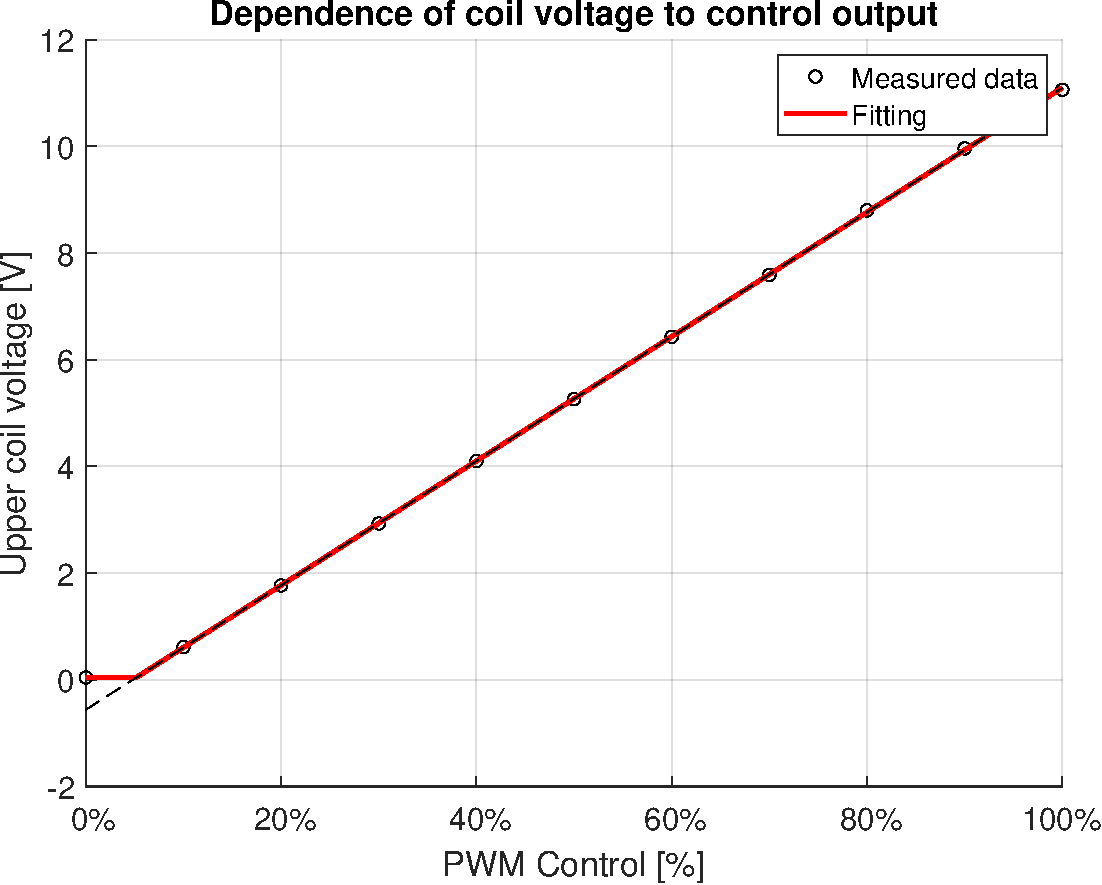
\includegraphics[width=0.6\textwidth]{img/MATLAB/measurements/control_to_voltage.pdf}
    \caption{Control to voltage identification}
    \label{fig:control_to_voltage}
\end{figure}

As we can see, the linear model for the relation $V_* = f(U) = f(\text{PWM})$ is a good approximation outside the initial black zone control.
Because of this, we can consider the following control to voltage relation:

\begin{equation}
    V_* = \begin{cases}
        V_{*min}    & \text{if } U < U_{min}    \\
        k_* U + c_* & \text{if } U \geq U_{min}
    \end{cases}
\end{equation}

Where $V_{*min}$ is the minimum voltage applied to the coils when the control signal is zero, $u_{min}$ is the minimum control signal that is effective on the voltage applied to the coils, $k_*$ is the slope of the linear model and $c_*$ is the offset of the linear model.

The values of the parameters are shown in Table \ref{tab:control_to_voltage_parameters}.

\begin{table}[H]

    \centering
    \begin{tabular}{|c|c|c|}
        \hline
        \textbf{Parameter} & \textbf{Value}            & \textbf{Units} \\
        \hline
        $V_{*min}$         & $4.300000 \cdot 10^{-2}$  & $V$            \\
        $U_{min}$          & $5.179276$                & $\%$           \\
        $k_*$              & $1.165800 \cdot 10^{1}$   & $V/\%$         \\
        $c_*$              & $-5.608000 \cdot 10^{-1}$ & $V$            \\
        \hline
    \end{tabular}

    \caption{Control to voltage identification parameters}
    \label{tab:control_to_voltage_parameters}

\end{table}


\subsubsection{Inductances characterization}
\label{subsubsec:inductances_characterization}

A key parameter of the system is the inductance of the coils.

As already proposed in Equation \ref{eq:model_for_inductance}, the inductance of the coils cannot be considered constant and both its dependence on the current and the position of the ball must be taken into account when dealing with the magnetic levitation system.

In order to identify the inductance of the coils and all the parameters needed to characterize them, we have to measure the values of $L_1$ and $L_2$ for many currents and ball positions.
Once we have these values, we can fit the data to the model proposed in Equation \ref{eq:model_for_inductance} and identify the parameters.

Given a certain (fix in time) position of the ball and a certain current step input, we can measure the value of the inductance of the coils, knowing that:

\begin{equation}
    V = R I + \frac{d (L I)}{d t} = R I + \left( \frac{\partial L}{\partial I} I + L \right) \dot{I}
\end{equation}

If we suppose for a moment that the variation of the inductance with the current is negligible, we can obtain a closed form solution for the current in the RL circuit as follows:

\begin{equation}
    I(t) = \frac{V_{max}}{R_0} \left( 1 - e^{- \frac{R_0}{L_0} t} \right)
    \label{eq:current_in_rl_circuit}
\end{equation}

Given the previous equation, we can adopt the following strategy to fully characterize the inductance of the coils over the range of possible ball positions and currents:

\begin{enumerate}
    \item Fix the ball at a certain height ($z^*$);
    \item Apply a certain current step input to the system ($I^*$);
    \item Measure the current in the coils ($I(t)$);
    \item Fit the measured current to the model proposed in Equation \ref{eq:current_in_rl_circuit} and identify $L(z^*, I^*)$;
    \item Repeat from step 2 for different step inputs of currents;
    \item Repeat from step 1 for different ball positions.
\end{enumerate}

In Figure \ref{fig:inductance_characterization_currents} we can see on the left all the dynamics of the current in the coils for different step inputs of currents and different ball positions, while on the right we can see the fitting of the data to the model proposed in Equation \ref{eq:current_in_rl_circuit}.

\begin{figure}[H]
    \centering
    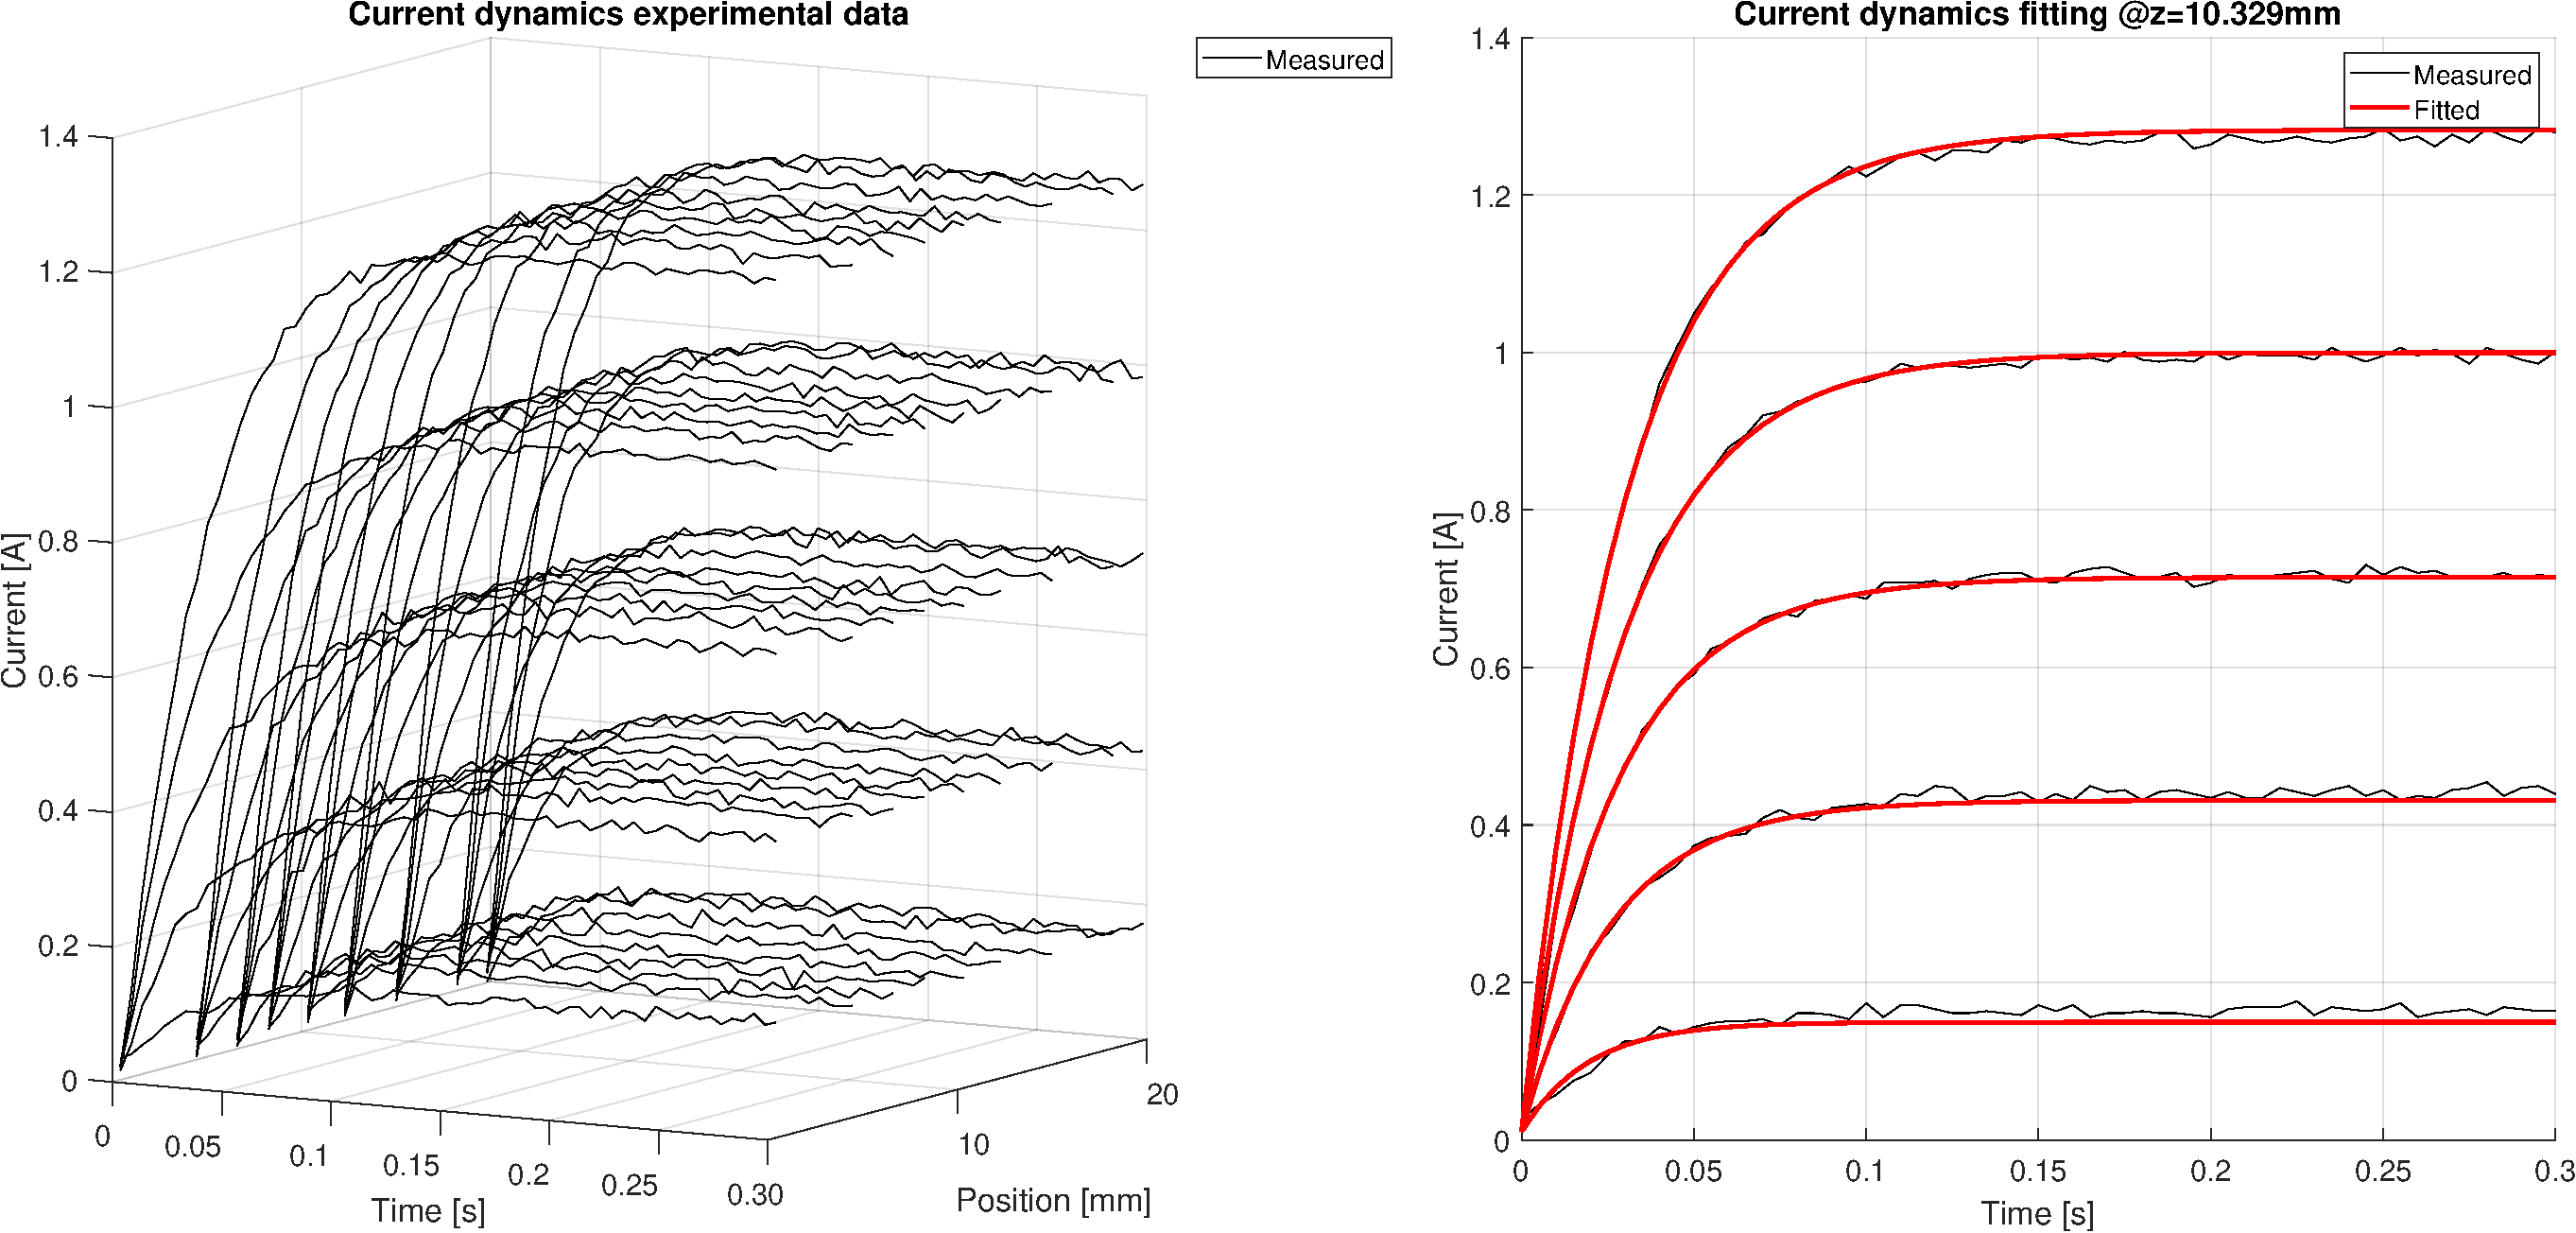
\includegraphics[width=1\textwidth]{img/MATLAB/measurements/currents.pdf}
    \caption{Inductance characterization for different currents and ball positions}
    \label{fig:inductance_characterization_currents}
\end{figure}

From the right side of Figure \ref{fig:inductance_characterization_currents} we can see that the fitting of the data to the model proposed in Equation \ref{eq:current_in_rl_circuit} is optimal for middle values of the current, while it tends to underestimate and overestimate the current for low and high values of the current, respectively.
This behavior is probably due to the fact that the variation of the inductance with the current that has been neglected in the model of the current (Equation \ref{eq:current_in_rl_circuit}) is not negligible and should have been taken into account.

Thanks to the data obtained from the multiple tests, we can now fit the values of the inductance of the coils to the model proposed in Equation \ref{eq:model_for_inductance} and identify the parameters.
The obtained model fitting is shown in Figure \ref{fig:inductance_characterization_inductance}.

\begin{figure}[H]
    \centering
    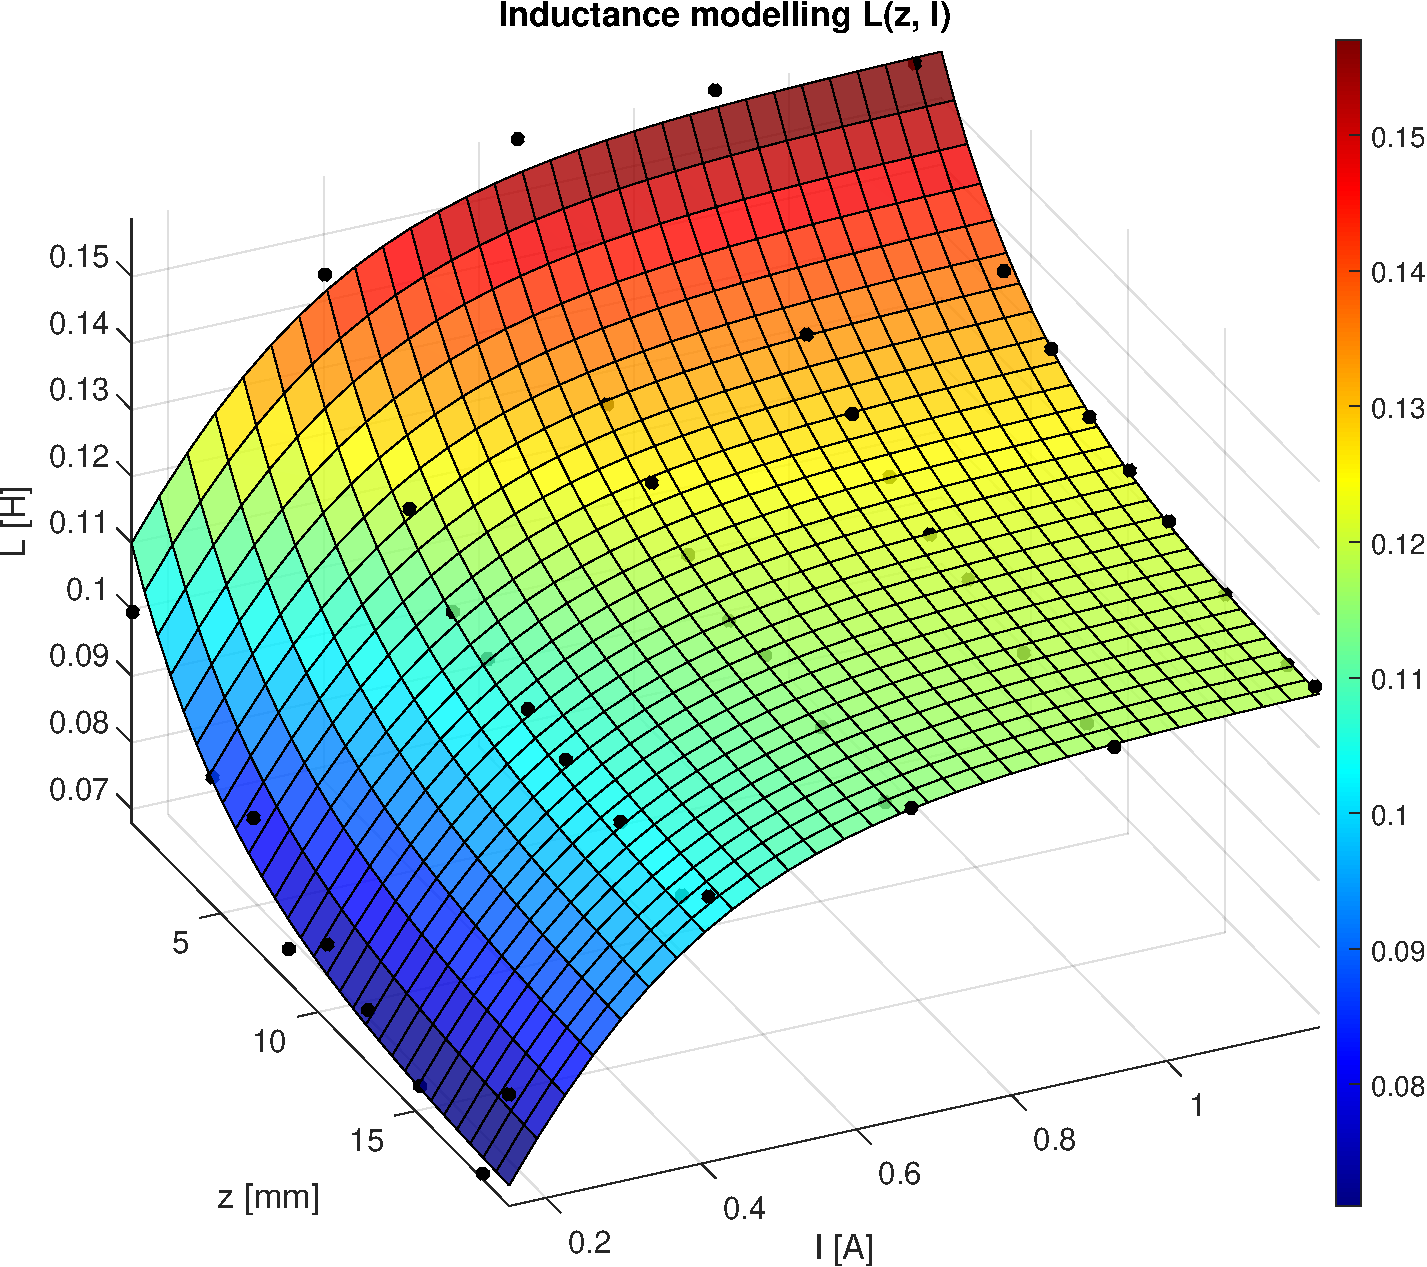
\includegraphics[width=0.6\textwidth]{img/MATLAB/measurements/inductance.pdf}
    \caption{Inductance characterization}
    \label{fig:inductance_characterization_inductance}
\end{figure}

One can clearly see the $90$ points that have been used to fit the model proposed in Equation \ref{eq:model_for_inductance} and the obtained fitting.
The values of the parameters are shown in Table \ref{tab:inductance_characterization_parameters}.

\begin{table}[H]
    \centering
    \begin{tabular}{|c|c|c|}
        \hline
        \textbf{Parameter} & \textbf{Value}  & \textbf{Units} \\
        \hline
        $L_0$              & $4.106763e-02$  & $H$            \\
        $a_z$              & $2.155909e+02$  & $1/m$          \\
        $L_z$              & $4.288065e-02$  & $H$            \\
        $a_I$              & $2.553122e+00$  & $1/A$          \\
        $L_I$              & $-7.675453e-02$ & $H$            \\
        \hline
    \end{tabular}

    \caption{Inductance characterization parameters}
    \label{tab:inductance_characterization_parameters}

\end{table}

\subsubsection{Force validation}
\label{subsubsec:force_validation}

The last test that we will perform is the force validation.

Thanks to the data obtained from the previous tests, we should already be able to predict the force applied to the ball by the inductance.
In particular, we already know that the electromagnetic force applied to the ball is given by the following equation:

\begin{equation}
    F_{em} = \frac{1}{2} \frac{\partial L}{\partial z} I^2
\end{equation}

Because of the previously identified parameters, we have an analytical expression for the sensitivity of the inductance with respect to the position of the ball.
However, due to uncertainties in the identification of the parameters, we can expect some discrepancies between the predicted force and the measured one.

In order to quantify these discrepancies and validate the model, we will use a direct method to measure the force applied to the ball by the inductance and compare it with the predicted one.
To do so, we recall Equation \ref{eq:reduced_equations_of_motion_final} and in particular the equation relative to $\dot{v}$:

\begin{equation}
    \dot{v} = m^{-1} \left(\frac{1}{2} \frac{\partial L_1}{\partial z} I_1^2 + \frac{1}{2} \frac{\partial L_2}{\partial z} I_2^2 + m g  \right)
\end{equation}

If we consider the system at rest, we can simplify the equation as follows:

\begin{equation}
    0 = \frac{1}{2} \frac{\partial L_1}{\partial z} I_1^2 + \frac{1}{2} \frac{\partial L_2}{\partial z} I_2^2 + m g
\end{equation}

Supposing now that only the first coil is energized, we can further simplify the equation as follows:

\begin{equation}
    0 = \frac{1}{2} \frac{\partial L_1}{\partial z} I_1^2 + m g
\end{equation}

Which leads to:

\begin{equation}
    \frac{\partial L_1}{\partial z} = -2 \frac{m g}{I_1^2}
    \label{eq:sensitivity_of_inductance}
\end{equation}

This last equation basically tells us that in steady state conditions, when the ball is levitating (i.e. $\dot{z} = 0$ and not supported by any platform), the sensitivity of the inductance of the first coil has an analytical expression that can be directly measured by measuring the current in the first coil.

In order to follow this approach, a linearly increasing voltage has been applied to the first coil and the current corresponding to the levitation of the ball has been measured.
The test has been repeated for different initial positions of the ball, in order to fully characterize the dynamic inductance characteristics over the range of possible ball positions.

In Figure \ref{fig:levitation_current} we can see both the position of the ball and the current circulating in the first coil.
By identifying the current at which the ball starts to levitate (i.e. the ball starts to move upwards), we can than use Equation \ref{eq:sensitivity_of_inductance} to identify the dynamic inductance characteristics.

\begin{figure}[H]
    \centering
    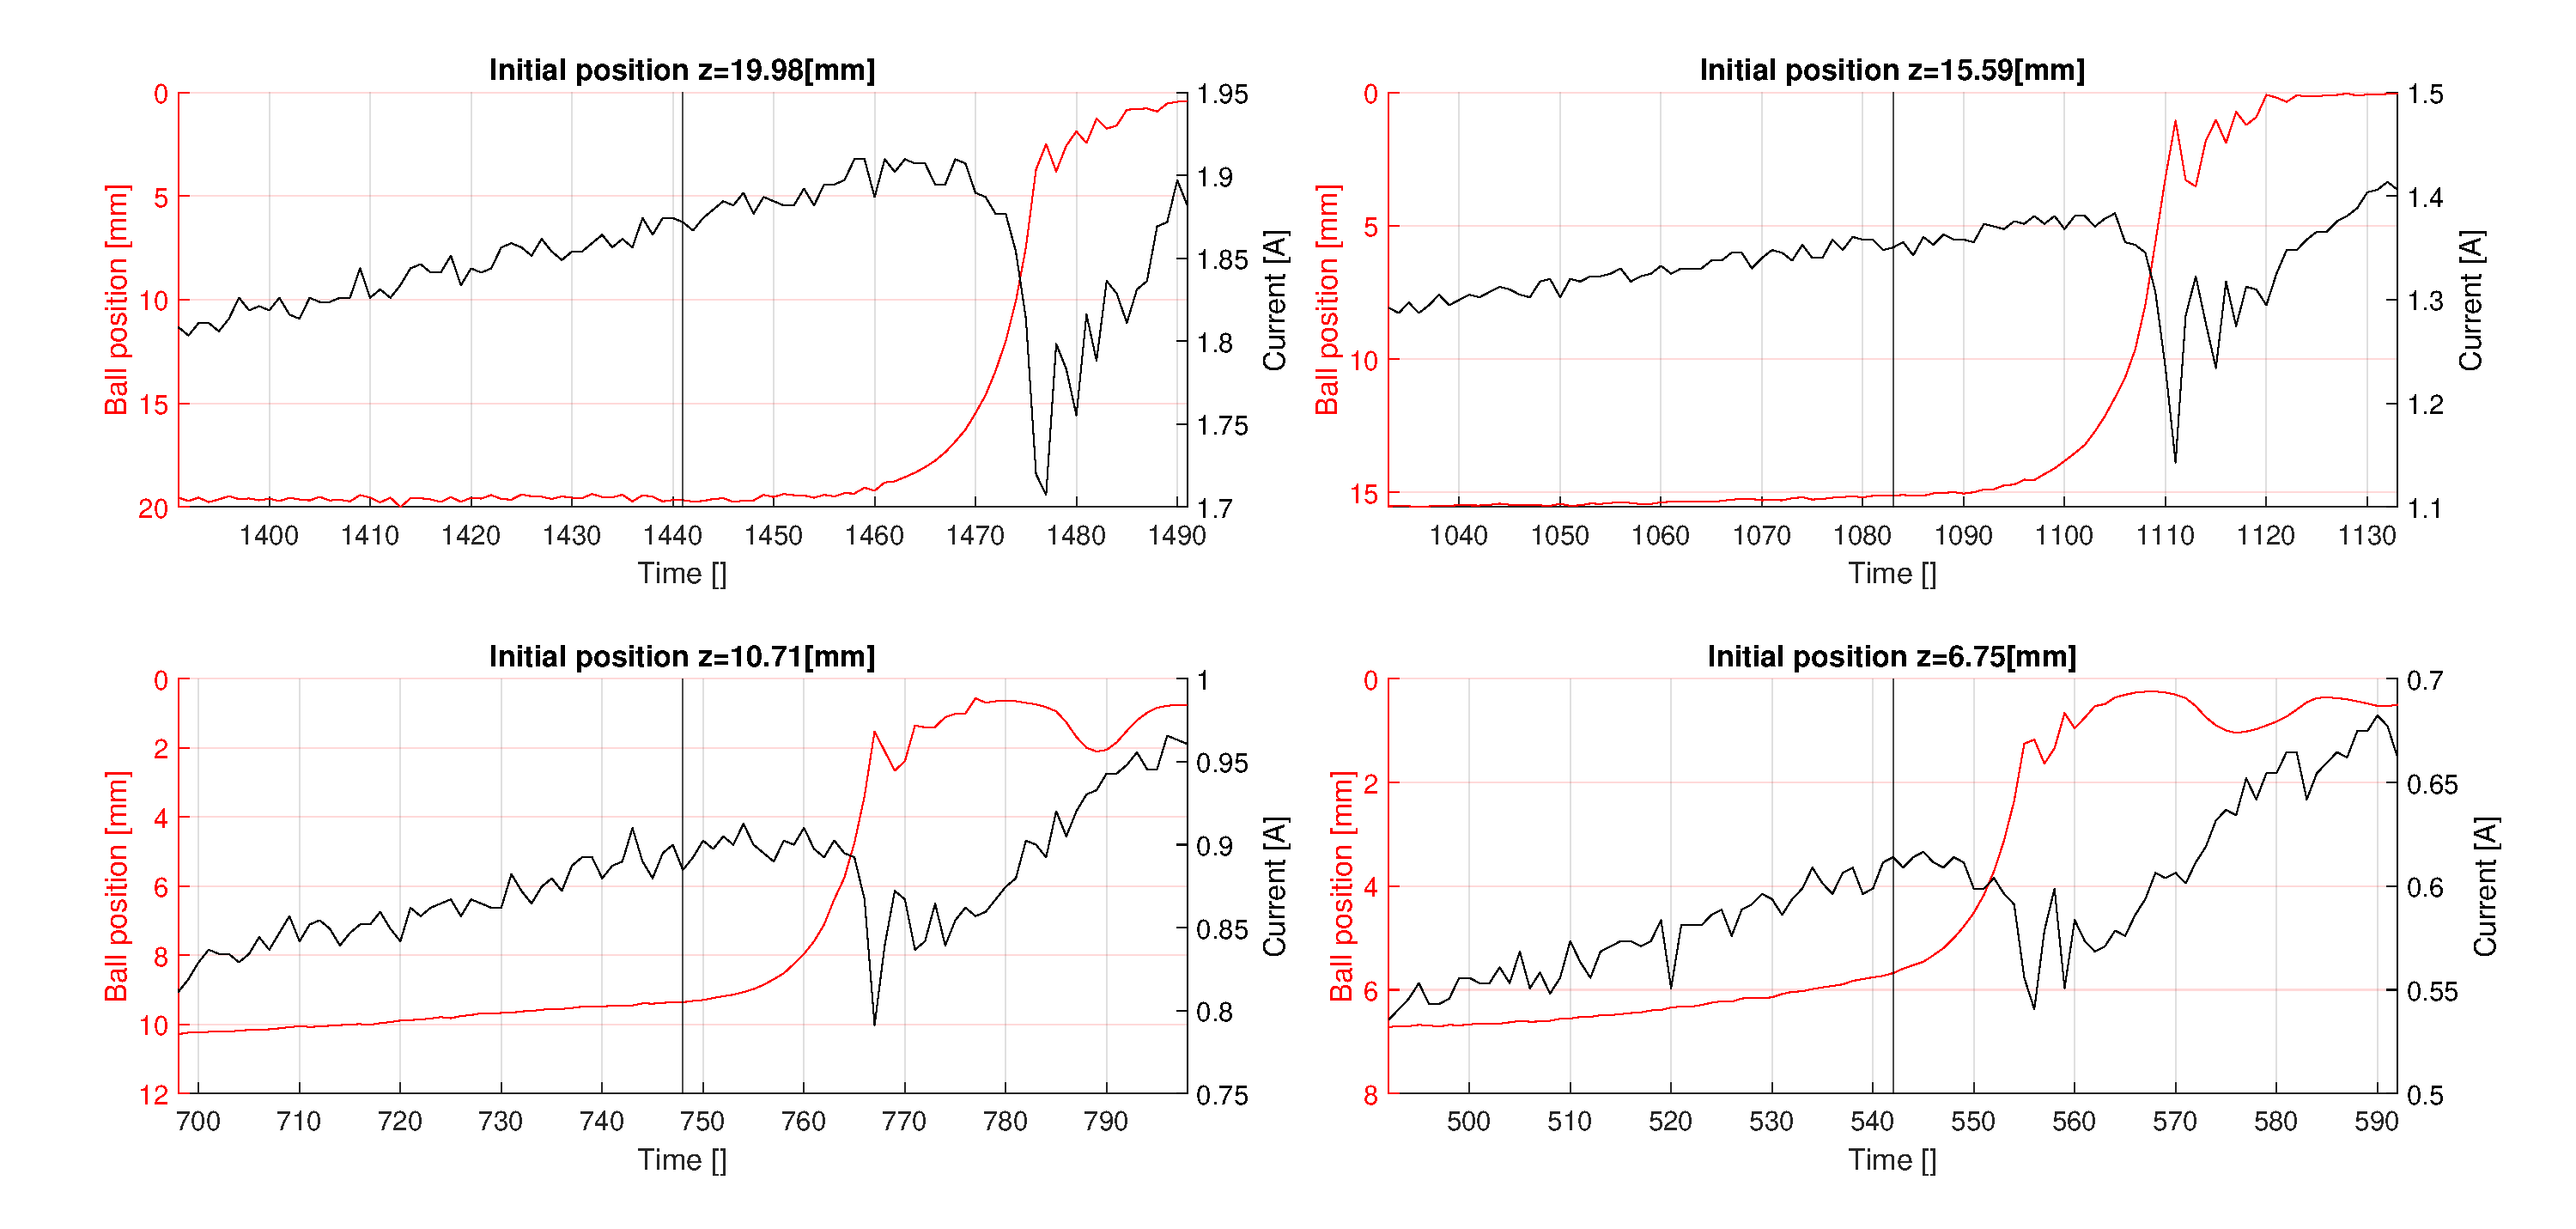
\includegraphics[width=1\textwidth]{img/MATLAB/measurements/currents_for_force.pdf}
    \caption{Position of the ball and current in the first coil around the levitation point (marked by vertical black line)}
    \label{fig:levitation_current}
\end{figure}

In Figure \ref{fig:dynamic_inductance_characteristics}, we can observe both the measured data and the fitted ones.
On the right side figure, a complete characterization of the electromagnetic force has been reconstructed based again on the above equations.

\begin{figure}[H]
    \centering
    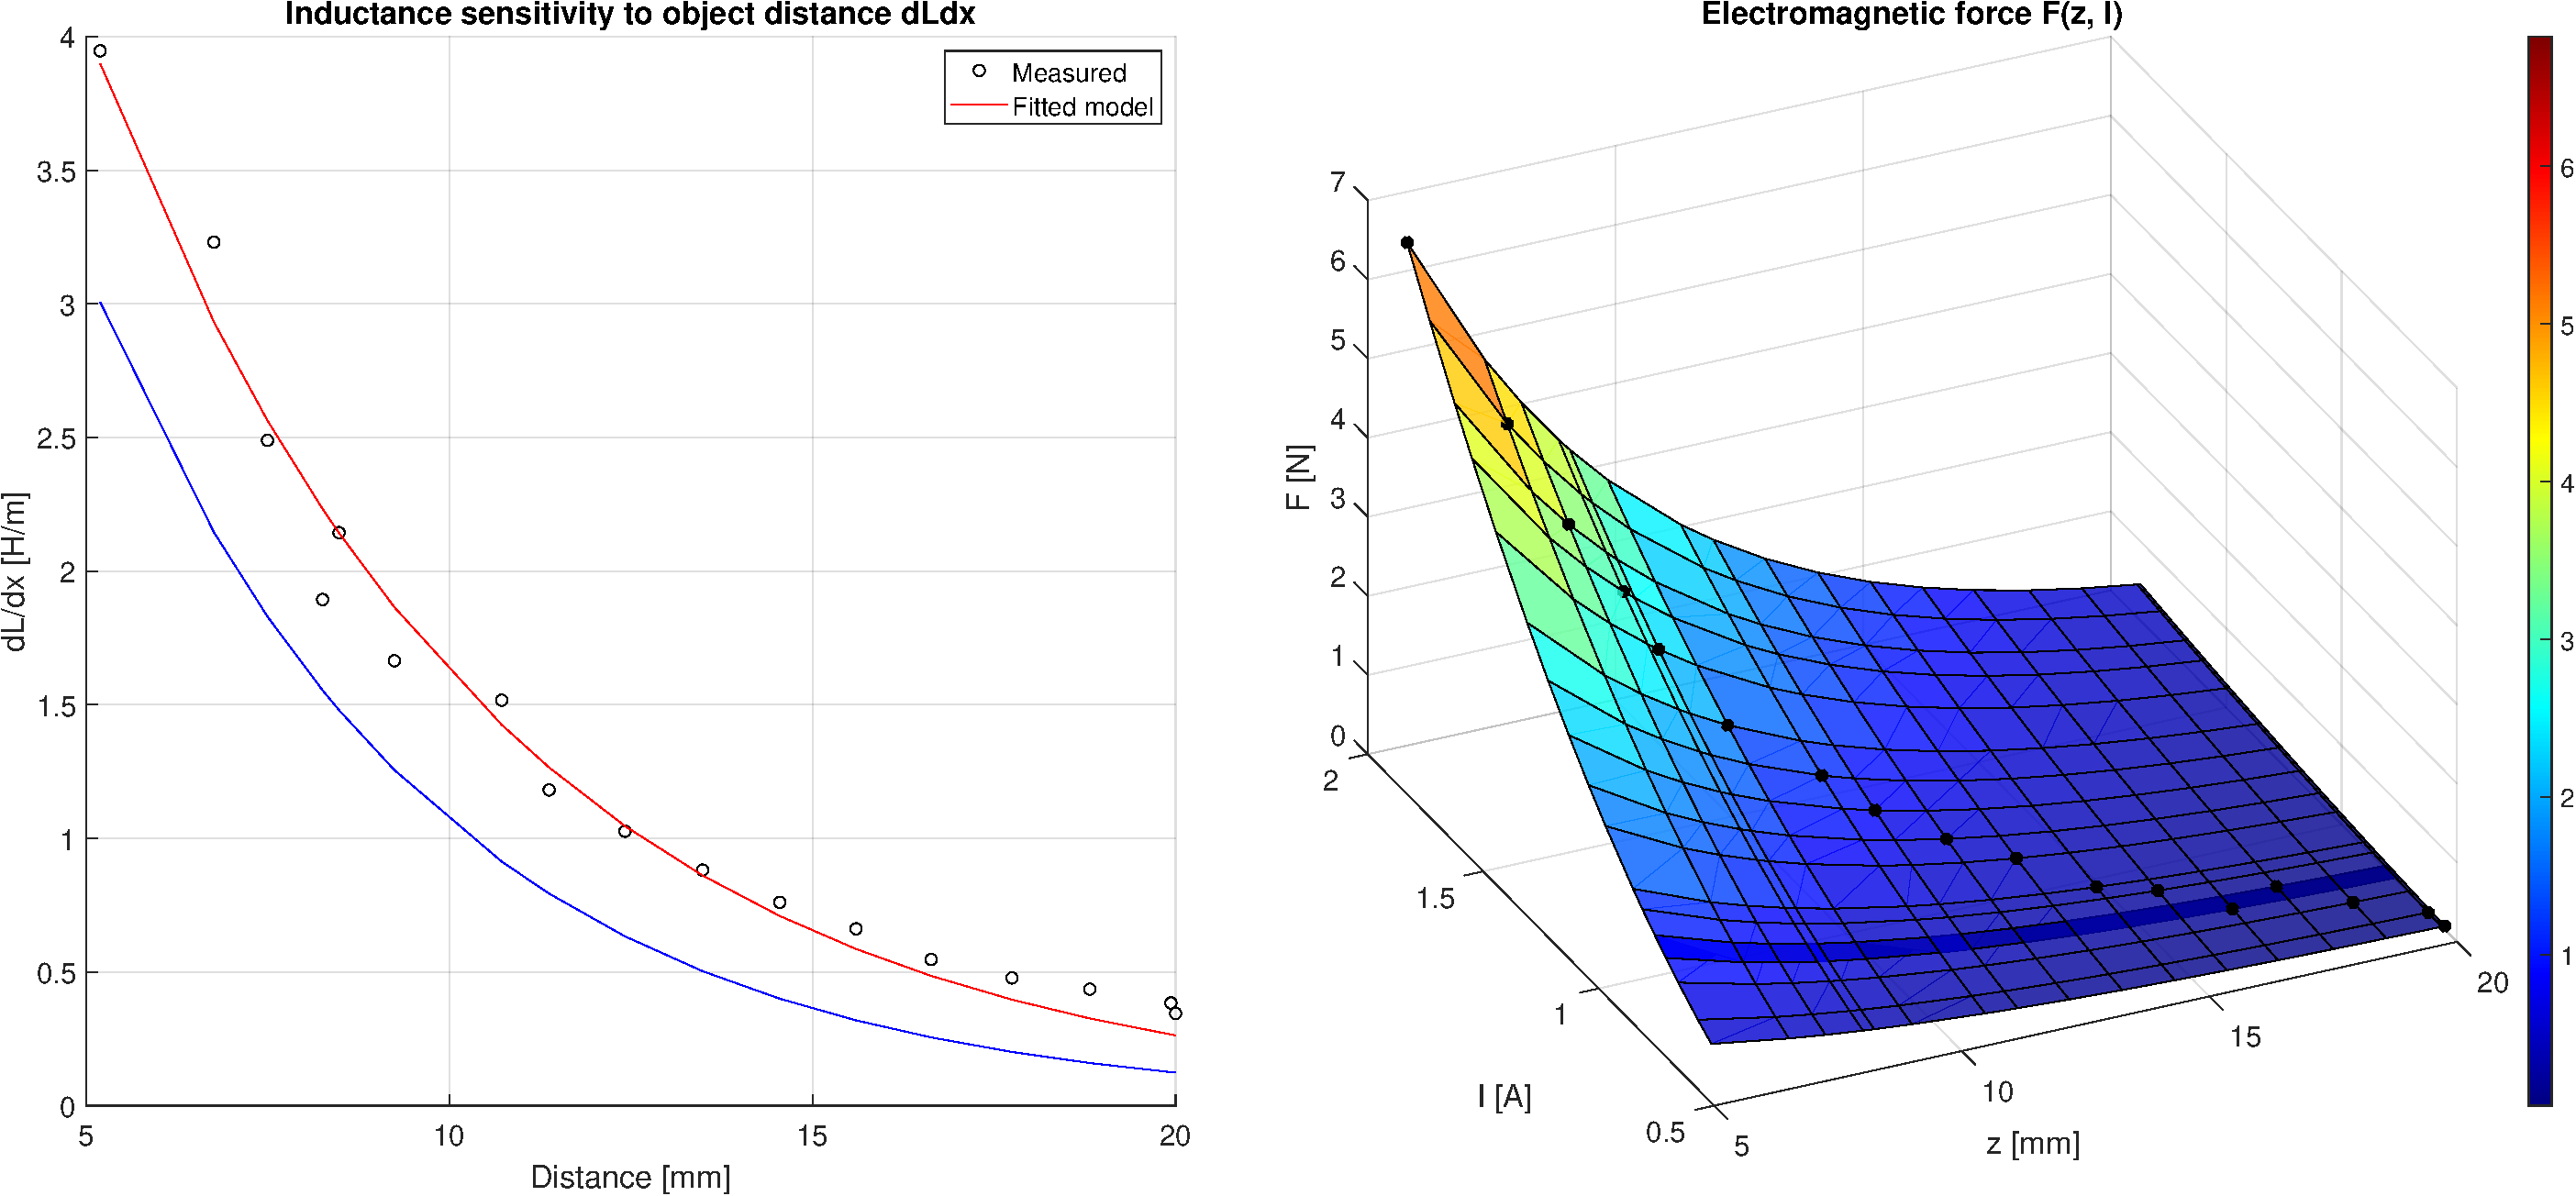
\includegraphics[width=1\textwidth]{img/MATLAB/measurements/force.pdf}
    \caption{Dynamic inductance characteristics and electromagnet force}
    \label{fig:dynamic_inductance_characteristics}
\end{figure}

As we can see,
